\chapter{Metodologia}
\label{cha:metodologia}

	O trabalho é executado a partir de revisão bibliográfica de textos acadêmicos, como dissertações e teses, artigos publicados em revistas acadêmicas, livros teóricos e notas de estudos técnicos. A revisão bibliográfica tem o objetivo de se inteirar do estado da arte das tecnologias envolvidas na Indústria 4.0.
	
	As disciplinas obrigatórias do programa de pós-graduação cursadas durante o período do mestrado foram selecionadas com base na relevância e relacionamento com a natureza da pesquisa em Indústria 4.0 e incluem disciplinas também de outros programas de pós-graduação, como o de Engenharia Elétrica, Engenharia de Transportes e Engenharia de Produção.
	
	A metodologia adotada neste projeto é baseada na proposta por \citeonline{jensen1997petrinet}, onde as etapas de pesquisa são compostas por um ciclo repetitivo de três aspectos, sendo elas: as teorias, as ferramentas e as aplicações; conforme ilustrado na \autoref{fig:metodologia-jensen}.
	
	O próprio conhecimento adquirido nas disciplinas por meio da aprendizagem de novas ``ferramentas'' pode modificar parte das ``aplicações'' e com isso realimentar as ``teorias'' iniciais. Mediante a evolução do projeto ao longo do tempo, novas propostas surgem, e com isso a necessidade do aprendizado de novos conceitos/teorias.

	\begin{figure}[htb]
		\centering
		\label{fig:metodologia-jensen}
		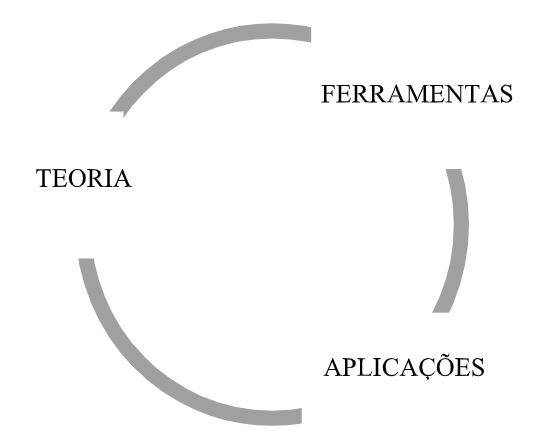
\includegraphics[width=0.7\textwidth]{metodologia-jensen.png}
		\caption{Metodologia de pesquisa utilizada.}
		\fonte{\citeonline{jensen1997petrinet} (adaptado).}
	\end{figure}

	Aplicando-se a metodologia proposta por \citeonline{jensen1997petrinet} para o caso específico da pesquisa em questão, pode-se listar teorias, ferramentas e aplicações individuais do projeto apresentadas em diferentes fases do projeto de pesquisa.
	
	A \autoref{fig:metodologia-jensen-projeto} mostra os elementos da metodologia de \citeonline{jensen1997petrinet} reformulados em diferentes fases do projeto: (a) na proposta inicial do projeto de pesquisa, (b) no relatório anual após um ano de pesquisa e (c) no texto para a qualificação do programa de mestrado.
	
	\begin{figure}[htb]
		\centering
		\label{fig:metodologia-jensen-projeto}
		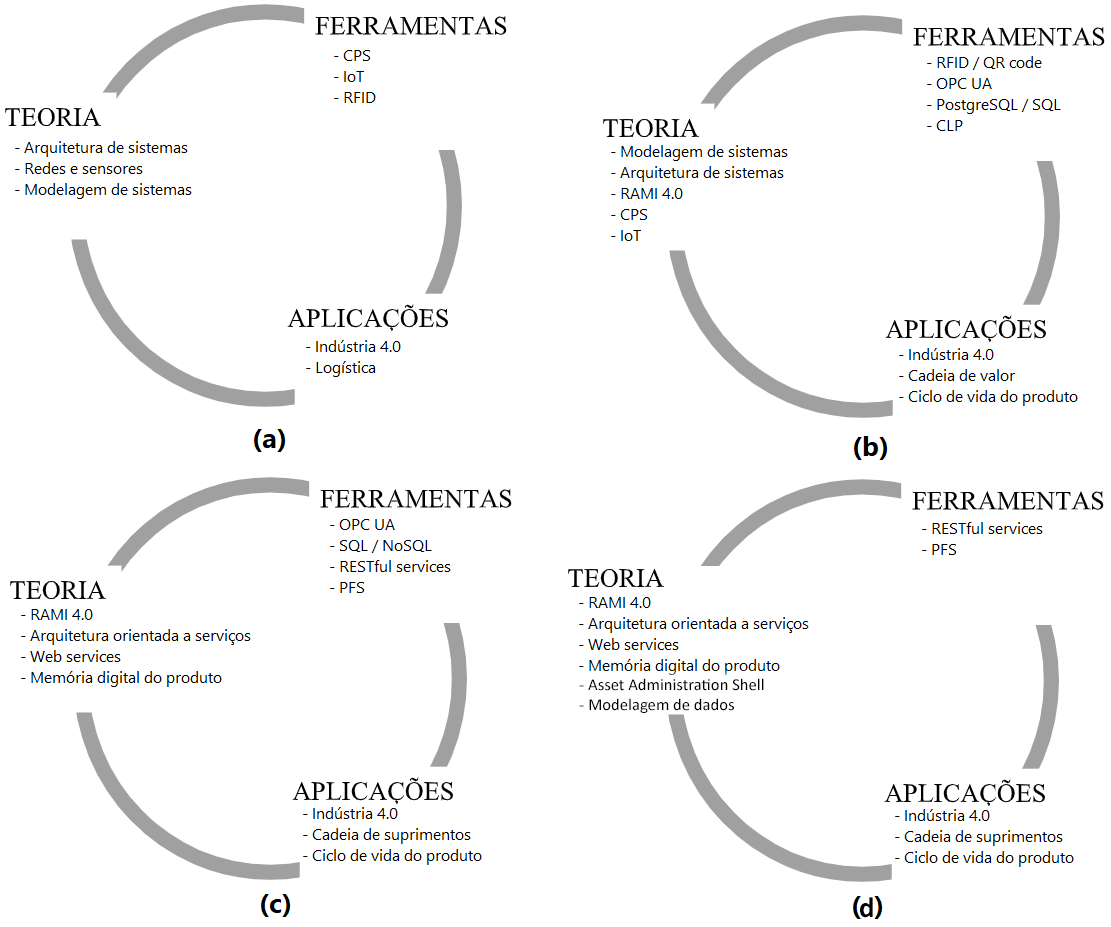
\includegraphics[width=1\textwidth]{metodologia-jensen-projeto.png}
		\caption{Teorias, ferramentas e aplicações apontadas em diferentes fases do projeto de pesquisa.}
	\end{figure}
	
	 Os ciclos mostrado na \autoref{fig:metodologia-jensen-projeto} se modificam constantemente à medida que o projeto de pesquisa evolui. Portanto, os três aspectos identificados no ciclo devem evoluir simultaneamente, recondicionando-se mutuamente.
